

\tikzset{every picture/.style={line width=0.75pt}} %set default line width to 0.75pt        

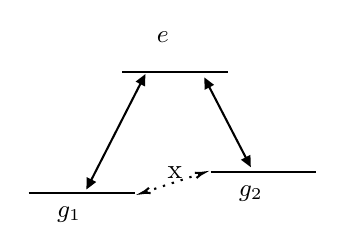
\begin{tikzpicture}[x=0.75pt,y=0.75pt,yscale=-1,xscale=1]
%uncomment if require: \path (0,121); %set diagram left start at 0, and has height of 121

%Straight Lines [id:da8945673509421989] 
\draw    (49,30) -- (99.97,30) ;
%Straight Lines [id:da9649284700544349] 
\draw    (4,88.23) -- (54.97,88.23) ;
%Straight Lines [id:da5481388569283493] 
\draw    (91.6,78.23) -- (142.57,78.23) ;
%Straight Lines [id:da8342940128052871] 
\draw    (58.83,33.73) -- (33.17,83.94) ;
\draw [shift={(31.8,86.61)}, rotate = 297.08] [fill={rgb, 255:red, 0; green, 0; blue, 0 }  ][line width=0.08]  [draw opacity=0] (5.36,-2.57) -- (0,0) -- (5.36,2.57) -- cycle    ;
\draw [shift={(60.2,31.06)}, rotate = 117.08] [fill={rgb, 255:red, 0; green, 0; blue, 0 }  ][line width=0.08]  [draw opacity=0] (5.36,-2.57) -- (0,0) -- (5.36,2.57) -- cycle    ;
%Straight Lines [id:da24634070519900753] 
\draw    (89.98,35.32) -- (109.62,73.2) ;
\draw [shift={(111,75.86)}, rotate = 242.59] [fill={rgb, 255:red, 0; green, 0; blue, 0 }  ][line width=0.08]  [draw opacity=0] (5.36,-2.57) -- (0,0) -- (5.36,2.57) -- cycle    ;
\draw [shift={(88.6,32.66)}, rotate = 62.59] [fill={rgb, 255:red, 0; green, 0; blue, 0 }  ][line width=0.08]  [draw opacity=0] (5.36,-2.57) -- (0,0) -- (5.36,2.57) -- cycle    ;
%Straight Lines [id:da9099096678817311] 
\draw  [dash pattern={on 0.84pt off 2.51pt}]  (86.7,79.08) -- (60.1,87.84) ;
\draw [shift={(58.2,88.46)}, rotate = 341.79] [color={rgb, 255:red, 0; green, 0; blue, 0 }  ][line width=0.75]    (4.37,-1.32) .. controls (2.78,-0.56) and (1.32,-0.12) .. (0,0) .. controls (1.32,0.12) and (2.78,0.56) .. (4.37,1.32)   ;
\draw [shift={(88.6,78.46)}, rotate = 161.79] [color={rgb, 255:red, 0; green, 0; blue, 0 }  ][line width=0.75]    (4.37,-1.32) .. controls (2.78,-0.56) and (1.32,-0.12) .. (0,0) .. controls (1.32,0.12) and (2.78,0.56) .. (4.37,1.32)   ;

% Text Node
\draw (64.2,9.17) node [anchor=north west][inner sep=0.75pt]  [font=\small]  {$\ket{e}$};
% Text Node
\draw (16.2,93.4) node [anchor=north west][inner sep=0.75pt]  [font=\small]  {$\ket{g_{1}}$};
% Text Node
\draw (103.8,83.4) node [anchor=north west][inner sep=0.75pt]  [font=\small]  {$\ket{g_{2}}$};
% Text Node
\draw (69.4,74.2) node [anchor=north west][inner sep=0.75pt]   [align=left] {x};


\end{tikzpicture}
